\documentclass[10pt,a4paper]{article}
\usepackage[utf8]{inputenc}
\usepackage[T1]{fontenc}
\usepackage{amsmath}
\usepackage{amsthm}
\usepackage{amssymb}
\usepackage{graphicx}
\usepackage{mathtools}
\usepackage[ruled,vlined,linesnumbered]{algorithm2e}
\usepackage[left=2.50cm, right=2.50cm, top=2.0cm, bottom=2.0cm]{geometry}


\makeatother
\DeclareMathOperator*{\argmin}{argmin}
\DeclareMathOperator*{\Max}{\text{max}}
\DeclareMathOperator*{\E}{\mathbb{E}}
\newcommand{\Ei}[1]{\mathbb{E}_{#1}}
\DeclareMathOperator*{\Eik}{\mathbb{E}_{\mathit{i_k}}}
\DeclareMathOperator*{\Eikplus}{\mathbb{E}_{\mathit{i_{k+1}}}}
\newcommand{\Eiplus}[1]{\mathbb{E}_{i_{#1}}}
\DeclareMathOperator*{\LC}{\text{\textup{LC}}^1}
\DeclareMathOperator*{\grad}{\mathit{\nabla \!f}}
\DeclareMathOperator*{\argmax}{arg\;max}
\DeclareMathOperator*{\gradik}{\mathit{\nabla\!\fik}}
\DeclareMathOperator*{\Lmax}{\mathit{L_{max}}}
\newcommand{\R}{\mathbb{R}}
\newcommand{\st}{\text{s.t.} \;\;\;}
\newcommand{\Rn}{\mathbb{R}^n}
\newcommand{\ikplus}{i_{k+1}}
\newcommand{\wrefi}[2]{w_{r(#1, i_{#2})}}
\newcommand{\wref}[1]{\wrefi{#1}{#1}}
\newcommand{\fik}{f_{i_k}}
\newcommand{\fikofwstar}{\fik(w^*)}
\newcommand{\fofwstar}{f(w^*)}
\newcommand{\fii}[1]{f_{i_{#1}}}
\newcommand{\fikplus}{f_{i_{k+1}}}
\newcommand{\fiplus}[1]{f_{i_{#1}}}
\newcommand{\fimax}{f_i^{\text{max}}}
\newcommand{\fikmax}{\fik^{\text{max}}}
\newcommand{\bmax}{b_{\text{max}}}
\newcommand{\fmax}{f^{\text{max}}}
\newcommand{\fmaxk}[1]{f_{i_{#1}}^{\text{max}}}
\newcommand{\Lik}{L_{i_k}}
\newcommand{\Cik}{C_{i_k}}
\newcommand{\deltak}{\delta^{l_k}}
\newcommand{\deltakplus}{\delta^{l_k+1}}
\newcommand{\deltakminus}{\delta^{l_k-1}}
\newcommand{\etatilde}{\tilde{\eta}_{k,0}}
\newcommand{\muik}{\mu_{i_k}}
\newcommand{\etamax}{\eta^{\text{max}}}
\newcommand{\etamaxx}{\bar{\eta}^{\text{max}}}
\newcommand{\etamin}{\eta^{\text{min}}}
\newcommand{\etaminn}{\bar{\eta}^{\text{min}}}
\newcommand{\minimum}[2]{\min \left\{ #1, #2 \right \} }
\newcommand{\maximum}[2]{\max \left\{ #1, #2 \right \} }
\newcommand{\W}[1]{{\scriptscriptstyle W #1}}
\newcommand{\gradi}[1]{\nabla f_{i_{#1}} (w_{i_{#1}}) }
\makeatletter

\newtheorem{assumption}{Assumption}
\newtheorem{lemma}{Lemma}
\newtheorem{proposition}{Proposition}
\newtheorem{theorem}{Theorem}
\newtheorem{corollary}{Corollary}
\newtheorem{remark}{Remark}


\newcommand{\imgS}{.26}
\newcommand{\dir}{exp1/}
\newcommand{\model}{mlp}
\newcommand{\modelname}{mlp}


\newcommand{\mlp}{{\texttt{mnist|mlp}}}
\newcommand{\res}{{\texttt{cifar10|resnet34}}}
\newcommand{\dense}{{\texttt{cifar10|densenet121}}}
\newcommand{\ress}{{\texttt{cifar100|resnet34}}}
\newcommand{\denses}{{\texttt{cifar100|densenet121}}}
\newcommand{\fashion}{{\texttt{fashion|effb1}}}
\newcommand{\svhn}{{\texttt{svhn|wrn}}}
\newcommand{\wiki}{{\texttt{wiki2|encoder}}}
\newcommand{\ptb}{{\texttt{ptb|xl}}}
\newcommand{\mushrooms}{{\texttt{mushrooms}}}
\newcommand{\rcvone}{{\texttt{rcv1}}}
\newcommand{\ijcnn}{{\texttt{ijcnn}}}
\newcommand{\weighta}{{\texttt{w8a}}}


\title{Optimization Methods}
\author{Chapter 3: Second-Order Methods for Unconstrained Optimization}
\date{}
\begin{document}
	\maketitle
	\section{Pure Newton Method}
	In the previous chapter, we have studied optimization problems like $\min_{x\in\Rn} f(x)$ with $f\in\C(\Rn)$, in particular, we only used first order information to build our methods. In this chapter we assume that $f\in\Cii(\Rn)$, and we will present second-order methods, that is, in addition to the information on function values and gradients, we will employ evaluations of the Hessian matrices. We will start from the most famous second-order method, namely Newton's method, whose main idea is the following. Given an iterate $x_k$, the next iterate $x_{k+1}$ is chosen to minimize the quadratic approximation of the function around $x_k$:
	\begin{equation*}
		x_{k+1} = \argmin_{x \in \mathbb{R}^n} q_k(x):= f(x_k) + \grad(x_k)^T (x - x_k) + \frac{1}{2}(x - x_k)^T \hess(x_k)(x - x_k).
	\end{equation*}
	The above update formula is not well-defined unless we further assume that $\hess(x_k)$ is positive definite. In that case, the unique minimizer of the minimization problem above is the unique stationary point:
	\begin{equation*}
		\grad(x_k) + \hess(x_k)(x_{k+1} - x_k) = 0,
	\end{equation*}
	which is the same as
	\begin{equation}\label{eq:newton}
		x_{k+1} = x_k - \hess(x_k)^{-1} \grad(x_k).
	\end{equation}
	The vector $-(\hess(x_k))^{-1} \grad(x_k)$ is called the Newton direction, and the algorithm induced by the update formula \eqref{eq:newton} is called the pure Newton's method. 
	
	\begin{algorithm}[H]\label{alg:newton}
		\caption{Pure Newton}
		
		\KwIn{Pick $x_0\in \Rn$ arbitrarly, $\epsilon>0$.}
		
		$k = 0$
		
		\While{$||\grad(x_k)||>\epsilon$}{
			
			Compute a direction $d_k$ as a solution to the linear system $\hess(x_k) d_k = -\grad(x_k)$
			
			$x_{k+1} = x_k +d_k$
			
			$k = k+1$
		}
	\end{algorithm}
\noindent Note that when $\hess(x_k)$ is positive definite for any $k$, Newton's directions are descent directions.
\begin{lemma}
	Let $f\in \Cii(\Rn)$ and let $\hess(x)\succ0,$ then $d_k = - \hess(x_k)^{-1} \grad(x_k)$ is a descent direction.
\end{lemma}
\begin{proof}
	That follows directly from the definition of $d_k$ and the fact that the inverse of a positive definite matrix is also positive definite, thus
	$\grad(x_k)^Td_k = - \grad(x_k)^T \hess(x_k)^{-1} \grad(x_k)<0.$ 
\end{proof}
\noindent By assuming that $\hess(x)$ is positive definite for every $x \in \mathbb{R}^n$ we also have that there exists a unique optimal solution $x^*$. However, this is not enough to guarantee convergence, as the following example illustrates.

\begin{example}
	Consider the function $f(x) = \sqrt{1 + x^2}$ defined over the real line. The minimizer of $f$ over $\mathbb{R}$ is of course $x = 0$. The first and second derivatives of $f$ are
	\begin{equation*}
		f'(x) = \frac{x}{\sqrt{1 + x^2}}, \quad f''(x) = \frac{1}{(1 + x^2)^{3/2}}.
	\end{equation*}
	Therefore, (pure) Newton's method has the form
	\begin{equation*}
		x_{k+1} = x_k - \frac{f'(x_k)}{f''(x_k)} = x_k - x_k(1 + x_k^2) = -x_k^3.
	\end{equation*}
	We therefore see that for $|x_0| \geq 1$ the method diverges and that for $|x_0| < 1$ the method converges very rapidly to the correct solution $x^* = 0$.
\end{example}
\noindent Even when it converges, its worst case rate is not better than that of GD, i.e., $\BigO(\epsilon^{-2})$.

\begin{definition}
	We say that $f\in \LCii(\Rn)$ if the Hessian is Lipschitz continuous, i.e., $ \exists\, L > 0$ for which $\|\hess(x) - \hess(y)\|_2 \leq L\|x - y\|$ for any $x, y \in \mathbb{R}^n$
\end{definition}
\begin{theorem}\label{thm:slow_newton}
	Algorithm \ref{alg:newton} applied to minimize a function $f\in \LC(\Rn)$ and $f\in \LCii(\Rn)$ bounded from below may require as many as $\epsilon^{-2}$ evaluations of $f$ and $\grad$ to produce an iterate $x\in \Rn$ such that $||\grad (x)\|\leq \epsilon.$
\end{theorem}
\begin{proof}
	Our aim is to build a function $f : \mathbb{R}^2 \to \mathbb{R}$ such that, for any $\epsilon \in (0,1)$, Newton's method takes at least $\epsilon^{-2}$ iterations to find an $\epsilon$-approximate first-order minimizer $x_\epsilon$ for which
	\begin{equation*}
		\|\grad(x_\epsilon)\| \leq \epsilon,
	\end{equation*}
	when started from the origin.\\
	Consider a hypothetical sequence of iterates $\{x_k\}_{k=0}^\infty$ such that $f(x_k) = f_k$, $\grad(x_k) = g_k$, and $\hess(x_k) = H_k$ are defined, for $k \geq 0$, by the relations
	\begin{equation}\label{eq:def_fk}
		f_k = 2 - k\epsilon^2, \quad g_k = \begin{pmatrix} -\epsilon^2 f_k \\ -\epsilon f_k \end{pmatrix}, \quad \text{and } H_k = \begin{pmatrix} \epsilon^2 f_k^2 & 0 \\ 0 & f_k^2 \end{pmatrix}.
	\end{equation}
	If this sequence of function, gradient, and Hessian values could be generated by Newton's method starting from the origin and applied to a function which is bounded from below, such that $f\in \LC(\Rn)$ and $f\in \LCii(\Rn)$, then for $k=0,\dots k_\epsilon$ with
	\begin{equation*}
		k_\epsilon \stackrel{\text{def}}{=} \left\lceil \epsilon^{-2} \right\rceil,
	\end{equation*}
	it is easy to check that
	\begin{equation*}
		f_k \in [1,2], \quad \|g_k\| = \epsilon f_k \sqrt{1 + \epsilon^2} > \epsilon, \quad \text{and } d_k = \frac{1}{f_k} \begin{pmatrix} 1 \\ \epsilon \end{pmatrix},
	\end{equation*}
	with the last equality resulting from \eqref{eq:newton}. As a consequence, this Newton iteration would require at least $k_\epsilon$ iterations (and evaluations of $f_k$, $g_k$, and $H_k$) before terminating. In addition,
	\begin{equation*}
		x_0 = \begin{pmatrix} 0 \\ 0 \end{pmatrix} \quad \text{and } x_k = \sum_{j=0}^{k-1} s_j. 
	\end{equation*}
	The next step in our construction is to build a smooth function with bounded second and third derivatives (which implies that its gradient and Hessian are Lipschitz continuous) interpolating \eqref{eq:def_fk} at $x_k$ as defined above. The idea is that $f(x)$ should behave exactly like its quadratic approximation $q_k$ around $x_k$. In particular, given 
	\begin{equation*}
		q_k(x) := f_k + g_k^T (x - x_k) + \frac{1}{2} (x - x_k)^T H_k (x - x_k),
	\end{equation*}
	we have $q_k(x_k) = f_k$, $\nabla q_k(x_k) = g_k$, and $\nabla^2 q_k(x_k) = H_k$. That also mean, that outside of this ball, the effects of all the other $q_k$ should be $0$. More precisely, for $k \geq 1$, let
	\begin{equation*}
		\sigma(\alpha) \stackrel{\text{def}}{=} \begin{cases}
			1 & \text{if } 0 \leq \alpha \leq \frac{1}{6}, \\
			1 + 27\left(\alpha - \frac{1}{6}\right)^3 \left[-10 + 45\left(\alpha - \frac{1}{6}\right) - 54\left(\alpha - \frac{1}{6}\right)^2\right] & \text{if } \frac{1}{6} \leq \alpha \leq \frac{1}{2}, \\
			0 & \text{if } \alpha \geq \frac{1}{2}.
		\end{cases}
	\end{equation*}
	This piecewise polynomial has the property that it is identically equal to 1 near the origin and to decrease smoothly to zero (with bounded first, second, and third derivatives) between $\frac{1}{6}$ and $\frac{1}{2}$ (Exercise: derive the formula for $\sigma$ with $\frac{1}{6}\leq \alpha\leq \frac{1}{2}$.). Using this function, we may then define, for each $k \geq 0$, a local support function $\sigma(\|x - x_k\|)$ that is identically equal to 1 in a (circular) neighbourhood of $x_k$ of radius $\frac{1}{6}$ and decreases smoothly (with bounded first, second, and third derivatives) to 0 for all points whose distance to $x_k$ exceeds $\frac{1}{2}$.
	We are now in a position to define the objective function as
	\begin{equation*}\label{eq:fSN}
		f_{SN}(x) = \sum_{k=0}^{k_\epsilon} \sigma(\|x - x_k\|) q_k(x)
	\end{equation*}
	for all $x$ in $\mathbb{R}^2$. Note that the sum in \eqref{eq:fSN} involves at most two nonzero terms for each $x$, because
	\begin{equation*}
		[d_k]_1 = 1/f_k > \frac{1}{2},
	\end{equation*}
	where we used the definition of $d_k$, and thus the distance between the first components of successive iterates (and thus also between the iterates themselves) exceeds $\frac{1}{2}$. This function, with its first two derivatives, obviously interpolates \eqref{eq:def_fk}, is bounded below, and has bounded first, second, and third derivatives since the large values of $q_k(x)$ that occur in their expressions always occur far from $x_k$ and are thus annihilated by the support function (verify everything as an Exercise). In particular, $f\in\LC(\Rn)$ and $f\in \LCii(\Rn)$.
\end{proof}

\begin{figure}
	\centering
	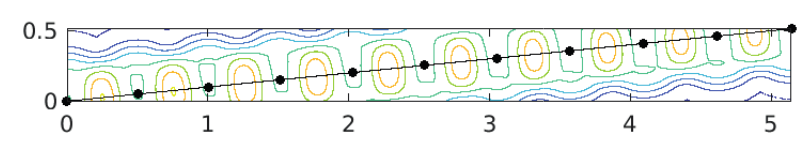
\includegraphics[width=0.5\linewidth]{slow_newton_contour}
	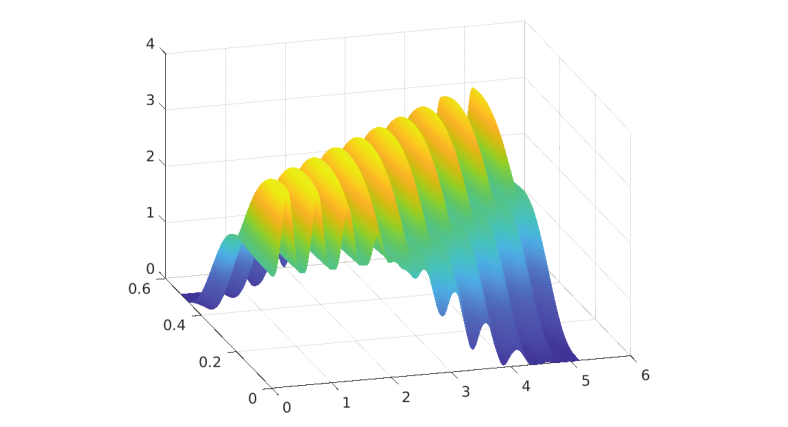
\includegraphics[width=0.5\linewidth]{slow_newton_3d}
	\caption{Contour lines of $f_{SN}(x)$ and the path of iterates for $k = 0, . . . , 10$. Below a 3D view of the function.}
\end{figure}
\noindent Despite all the negative results listed here, Newton's method does have one very attractive feature: one can prove local quadratic rate of convergence, which means that near the optimal solution the errors $e_k = \|x_k - x^*\|$ (where $x^*$ is the unique optimal solution) satisfy the inequality $e_{k+1} \leq M e_k^2$ for some positive $M > 0$. This property essentially means that the number of accuracy digits is doubled at each iteration.

\begin{theorem}[Quadratic local convergence of Newton's method]\label{thm:newton}
	Let $f\in \Cii(\Rn)$ with $\hess$ Lipschitz continuous. Moreover, let $\hess(x)$ be positive definite for any $x \in \mathbb{R}^n$. Let $\{x_k\}_{k \geq 0}$ be the sequence generated by Algorithm \ref{alg:newton}, and let $x^*$ be the unique minimizer of $f$ over $\mathbb{R}^n$. Then, we have 
	\begin{equation}\label{eq:newton_contraction}
		\|x_{k+1} - x^*\| \leq \frac{L}{2m}\|x_k - x^*\|^2 \quad \forall k = 0, 1, \ldots
	\end{equation}
	holds. In addition, if $\|x_0 - x^*\| \leq \frac{m}{L}$, then
	\begin{equation}\label{eq:local_newton}
		\|x_k - x^*\| \leq \frac{2m}{L} \left(\frac{1}{2}\right)^{2^k}.
	\end{equation}
\end{theorem}
\begin{proof}
	Let $k$ be a nonnegative integer. Then, from  $\grad(x^*)=0$ and the fundamental Theorem of Calculus, we have
	\begin{align*}
		x_{k+1} - x^* &= x_k - (\hess(x_k))^{-1} \grad(x_k) - x^* \nonumber \\
		&= x_k - x^* + (\hess(x_k))^{-1}(\grad(x^*) - \grad(x_k)) \nonumber \\
		&= x_k - x^* + (\hess(x_k))^{-1} \int_0^1 [\hess(x_k + t(x^* - x_k))](x^* - x_k) dt \nonumber \\
		&= (\hess(x_k))^{-1} \int_0^1 [\hess(x_k + t(x^* - x_k)) - \hess(x_k)](x^* - x_k) dt. \nonumber
	\end{align*}
	Combining the latter equality with the fact that $\hess(x)\succ 0 \forall x,$ i.e., $\exists m>0: \hess(x_k) \succeq mI$, implies that $\|(\hess(x_k))^{-1}\| \leq \frac{1}{m}$. Hence,
	\begin{align*}
		\|x_{k+1} - x^*\| &\leq \|(\hess(x_k))^{-1}\| \left\| \int_0^1 [\hess(x_k + t(x^* - x_k)) - \hess(x_k)](x^* - x_k) dt \right\| \nonumber \\
		&\leq \|(\hess(x_k))^{-1}\| \int_0^1 \left\| [\hess(x_k + t(x^* - x_k)) - \hess(x_k)](x^* - x_k) \right\| dt \nonumber \\
		&\leq \|(\hess(x_k))^{-1}\| \int_0^1 \|\hess(x_k + t(x^* - x_k)) - \hess(x_k)\| \cdot \|x^* - x_k\| dt \nonumber \\
		&\leq \frac{L}{m} \int_0^1 t \|x_k - x^*\|^2 dt = \frac{L}{2m} \|x_k - x^*\|^2, \nonumber
	\end{align*}
where the last inequality follows from the Lipschitz continuity of the Hessian.	Now, we will prove inequality \eqref{eq:local_newton} by induction on $k$. Note that for $k = 0$, we assumed that
	\begin{equation*}
		\|x_0 - x^*\| \leq \frac{m}{L},
	\end{equation*}	
	so in particular
	\begin{equation*}
		\|x_0 - x^*\| \leq \frac{2m}{L} \left(\frac{1}{2}\right)^{2^0},
	\end{equation*}
	establishing the basis of the induction. Assuming that \eqref{eq:local_newton} holds for an integer $k$, that is, $\|x_k - x^*\| \leq \frac{2m}{L} \left(\frac{1}{2}\right)^{2^k}$, we will show it holds for $k + 1$. Indeed, by \eqref{eq:newton_contraction} we have
	\begin{equation*}
		\|x_{k+1} - x^*\| \leq \frac{L}{2m} \|x_k - x^*\|^2 \leq \frac{L}{2m} \left(\frac{2m}{L} \left(\frac{1}{2}\right)^{2^k}\right)^2 = \frac{2m}{L} \left(\frac{1}{2}\right)^{2^{k+1}},
	\end{equation*}
	proving the desired result.
\end{proof}
\begin{remark}
	To compare Theorems \ref{thm:slow_newton} and \ref{thm:newton} it is important to notice that \eqref{eq:def_fk} is singular for $\epsilon\to 0$ otherwise, because of Theorem \ref{thm:newton}, the algorithm would achieve quadratic local convergence.
\end{remark}
\noindent Now, in order to ensure \textbf{global convergence} and maintain the local property of Theorem \ref{thm:newton}, we can employ one of the following globalization techniques:
\begin{itemize}
	\item \textbf{Line search} techniques applied to a descent direction constructed from Newton's direction;
	\item \textbf{Trust region} methods, where $s_k$ is chosen as the optimal solution (with a certain degree of approximation) of
	\begin{equation*}
		\min_{\|d_k\| \leq \Delta_k} q_k(d_k), \quad \with d_k:=x-x_k
	\end{equation*}
	appropriately updating the trust region radius $\Delta_k$ along the iterations (approximations of $\hess(x_k)$ can be used);
	\item \textbf{Regularized} methods, where $d_k$ is chosen as the optimal solution (with a certain degree of approximation) of
	\begin{equation*}
		\min_{d_k \in \mathbb{R}^n} q_k(d_k) + \sigma_k \|d_k\|^3
	\end{equation*}
	appropriately updating $\sigma_k$ along the iterations (approximations of $\hess(x_k)$ can be used).
\end{itemize}



\section{Line Search-based Newton method}
The Theorem \ref{thm:newton} above can be relaxed as follows. First of all, we don't need the Hessian to be positive definite in each $x\in \Rn$, but we just need to be able to invert it in $x^*$ and (by continuity) in a ball around it. Moreover, instead of solving the Newton equation \eqref{eq:newton} exactly, we can do it inexactly.
\begin{proposition}[Local Convergence of Inexact Newton]\label{inexact_newton}
	Let $f\in \Cii(\mathcal{D})$ where $\mathcal{D} \subseteq \mathbb{R}^n$ is an open set. Suppose that the following conditions hold:
	\begin{itemize}
		\item[(i)] there exists a point $x^* \in \mathcal{D}$ such that $\grad(x^*) = 0$;
		\item[(ii)] the Hessian matrix $\hess(x^*)$ is non singular.
	\end{itemize}
	Then, there exist an open ball $\mathcal{B}(x^*; r) \subset \mathcal{D}$, and a value $\bar{\eta}$ such that, if $x_0 \in \mathcal{B}(x^*; r)$ and $\eta_k \in [0, \bar{\eta}]$ for all $k$, then the sequence $\{x_k\}$ generated by the inexact Newton method and defined by the iteration $x_{k+1} = x_k + d_k$, where $d_k$ satisfies the condition
	\begin{equation}\label{eq:truncated_Newton}
		\| \nabla q_k(d_k)\|=\|\hess(x_k) d_k + \grad(x_k)\| \leq \eta_k \|\grad(x_k)\|,
	\end{equation}
	converges to $x^*$ with linear convergence rate. Moreover 
	\begin{itemize}
		\item[(a)] if $\eta_k \to 0$ then $\{x_k\}$ converges with superlinear convergence rate, i.e., 
		$$ \lim_{k\to \infty} \frac{||x_{k+1}-x^*||}{||x_k-x^*||}=0;$$
		\item[(b)] if $f\in \LCii(\mathcal{D})$, and there exists a constant $C > 0$ such that $\eta_k \leq C \|\grad(x_k)\|$ for all $k$, then $\{x_k\}$ converges with quadratic convergence rate.
	\end{itemize}
\end{proposition}

\noindent In case the solution of the Newton equation is constructed via an iterative procedure which is  interrupted when is \eqref{eq:truncated_Newton} is satisfied, the resulting method is called Truncated Newton (TN).

At this point, we have studied an iterative method which solves linear system of equation, i.e., Conjugate Gradient. Thus, we can apply it to find $d_k$, however, as in the general case the Hessian matrix $\hess(x_k)$ may be not positive definite, we need to suitably adapt CG to determine a descent direction.

In the following algorithm we omit the iteration counter $k$ inside the CG procedure (all the variables there should actually have both the $k$ and $i$ subscripts).\\
\begin{algorithm}[H]\label{alg:tncg}
\caption{Truncated Newton with Conjugate Gradient (TNCG)}

\KwIn{Pick $x_0\in \Rn$ arbitrarly, $\eta > 0$, $\epsilon > 0$, $\epsilon_2 > 0$}

$k=0$

\While{$||\grad(x_k)|| > \epsilon$}{
	
	$i = 0$, $d_0 = 0$, $s_0 = -\nabla q_0 = -\grad(x_k)$
	
	\While{True}{
		
		\If{$s_i^T \hess(x_k) s_i \leq \epsilon_2 \|s_i\|^2$}{		
		
			$d_k = \begin{cases}
				-\grad(x_k), & \text{if } i = 0, \\
				d_i, & \text{if } i > 0
			\end{cases}$
	
			\textbf{break}
		}
	
		$\alpha_i = -\frac{\nabla q_i^T s_i}{s_i^T \hess(x_k) s_i}$
		
		$d_{i+1} = d_i + \alpha_i s_i$
		
		$\nabla q_{i+1} = \nabla q_i + \alpha_i \hess(x_k) s_i.$
		
		\If{$\|\nabla q_i\| \leq \eta \|\grad(x_k)\| \min\left\{\frac{1}{k+1}, \|\grad(x_k)\|\right\}$}{
			
			$d_k = d_i$
			
			\textbf{break}
		}
	
		$\beta_{i+1} = \frac{\nabla q_{i+1}^T \hess(x_k) s_i}{s_i^T \hess(x_k) s_i}$
		
		$s_{i+1} = -\nabla q_{i+1} + \beta_{i+1} s_i,$
		
		$i= i+1$
	}
	
	$t_k \leftarrow$ Line Search along $d_k$ with 1 as initial step.
	
	$x_{k+1} = x_k +t_k d_k$
	
	$k = k+1$
}
\end{algorithm}
\noindent Regarding Step 10 above, from (39) of Chapter 2 we would get 
$\grad(x_{k+1}) = \grad(x_k) +\alpha_k Q d_k$ which when applied to $q_{k,i}(s_i)$ as an internal procedure becomes exactly $\nabla q_{i+1} = \nabla q_i + \alpha_i \hess(x_k) s_i.$
\par Given that $d_{k,0}=-\grad(x_k)$, CG is iteratively refining a gradient direction into a Newton direction (see Proposition \ref{inexact_newton}).

\begin{proposition}\label{prop:truncated_newton}
	Let $f \in \LC(\Rn)$ and $f\in \Cii(\Rn)$. Let $\{x_k\}$ and $\{d_k\}$ be the sequences generated by Algorithm \ref{alg:tncg}. There exist two numbers $c_1 > 0$ and $c_2 > 0$ such that for all $k$ we have
	\begin{equation}\label{eq:gradient_related}
		\begin{split}
			\grad(x_k)^T d_k &\leq -c_1 \|\grad(x_k)\|^2 \\
			\|d_k\| &\leq c_2 \|\grad(x_k)\|. 
		\end{split}
\end{equation}
\end{proposition}
\begin{proof}
	
%Notice that \eqref{eq:newton} can be transformed into a quadratic optimization problem, thus all the relationship derived for that method still hold here.
From Step 10, we have
\begin{equation*}
	\nabla q_i = \nabla q_0 + \sum_{j=0}^{i-1} \alpha_j \hess(x_k) s_j.
\end{equation*}
and consequently
\begin{equation*}
	\alpha_i = -\frac{\nabla q_i^T s_i}{s_i^T \hess(x_k) s_i} = - \frac{\nabla q_0^T s_i}{s_i^T \hess(x_k) s_i}.
\end{equation*}
because all the vectors $s_j$ are mutually $\hess(x_k)$-conjugate. Now let $d_k$ be the direction computed by Algorithm \ref{alg:tncg}. By construction, either $d_k = -\grad(x_k)$ or $d_k = d_i$. In the second case, we have that 
\begin{equation}\label{eq:positive_definite}
	s_j^T \hess(x_k) s_j>0 \quad \forall j < i,
\end{equation}
and we can write
\begin{equation*}
d_k = d_i = \sum_{j=0}^{i-1} \alpha_j s_j = -\sum_{j=0}^{i-1} \frac{\nabla q_0^T s_j}{s_j^T \hess(x_k) s_j} s_j,
\end{equation*}
from which, recalling that in the algorithm we have
\begin{equation*}
\nabla q_0 = \grad(x_k), \quad s_0 = -\grad(x_k),
\end{equation*}
and, from \eqref{eq:positive_definite}, also
\begin{equation*}
\grad(x_k)^T d_k = -\sum_{j=0}^{i-1} \frac{(\grad(x_k)^T s_j)^2}{s_j^T \hess(x_k) s_j} \leq -\frac{(\grad(x_k)^T \grad(x_k))^2}{\grad(x_k)^T \hess(x_k) \grad(x_k)}.
\end{equation*}
It follows that $\grad(x_k)^T d_k < 0$, furthermore we can write
\begin{equation*}
|\grad(x_k)^T d_k| \geq \frac{\|\grad(x_k)\|^4}{\|\grad(x_k)\|^2 \|\hess(x_k)\|} \geq \frac{1}{L} \|\grad(x_k)\|^2,
\end{equation*}
as $f\in \LC(\Rn)$ is equivalent to $\|\hess(x)\|\leq L \; \forall x\in \Rn$. Taking into account that we can have $d_k = -\grad(x_k)$, we can conclude that the first inequality in \eqref{eq:gradient_related} is satisfied with $c_1 \leq \min\{1, 1/L\}$. Concerning the second inequality in \eqref{eq:gradient_related}, if $d_k = d_i$ then we have
\begin{equation*}
\|d_k\| = \|d_i\| \leq \sum_{j=0}^{i-1} \left|\frac{||s_j||^2}{s_j^T \hess(x_k) s_j}\right| \|\grad(x_k)\|,
\end{equation*}
and hence, since we must have
\begin{equation*}
s_j^T \hess(x_k) s_j > \epsilon_2 \|s_j\|^2,
\end{equation*}
we obtain 
$$\|d_i\|\leq \frac{i}{\epsilon}||\grad(x_k)||\leq\frac{n}{\epsilon} \|\grad(x_k)\|,$$
where the last inequality comes from the fact that either CG has only encountered $n$ vectors $s_j$ for which $s_j^T \hess(x_k) s_j >0$, and consequently it terminates because of Proposition 9.2 from Chapter 2 within $n$ iterations, or it encountered a vector for which $s_j^T \hess(x_k) s_j<0$ before. This brings to the second inequality in \eqref{eq:gradient_related} with $c_2:=\max\{1,\frac{n}{\epsilon}\}$.
\end{proof}

\noindent Directions $d_k$ that satisfy \eqref{eq:gradient_related} are called \textbf{gradient-related} and they satisfy the \textbf{angle condition} with $c=\frac{c_1}{c_2}$, i.e., the cosine between the gradient and the direction is obtuse
$$ 	\frac{\grad(x_k)^T d_k}{\|d_k\|\|\grad(x_k)\|} \leq -c.$$
Once we have Proposition \ref{prop:truncated_newton}, we can achieve global convergence if we notice the following. 
\begin{lemma} Let $f\in \LC(\Rn)$. Assume that $d_k$ satisfy \eqref{eq:gradient_related} with certain $c_1, c_2>0$, then a Line Search method on $x_k$ along $d_k$ with initial step size 1 terminates in a finite amount iteration with $t_k\geq \min \{1, \frac{2c_1(1-\alpha)\beta}{Lc_2^2}\}.$
\end{lemma}
\begin{proof}
	Exercise, it follows from \eqref{eq:gradient_related} and from the Descent Lemma (part 1).
\end{proof}
\begin{corollary}
	The iteration complexity of Algorithm \ref{alg:tncg} is $\BigO(\epsilon^{-2})$.
\end{corollary}
\begin{proof}
	Exercise, it follows from the line search condition.
\end{proof}
\begin{remark}
	The relaxation proposed in Proposition \ref{prop:truncated_newton}, obviously does not solve the slow convergence proved in Theorem \ref{thm:slow_newton} for the pure Newton method. In fact, when the directions have a negative curvature, the solution proposed by Algorithm \ref{alg:tncg} is to fall back on a gradient-like direction, which also have a $\BigO(\epsilon^{-2})$ iteration complexity. 
\end{remark}
\noindent Notice that in Proposition \ref{prop:truncated_newton}, we assume that $x_{k+1} = x_k + d_k$, while in Algorithm \ref{alg:tncg} we need to employ a line search technique to ensure a sufficient decrease. This may cut the Newton step $d_k$ possibly slowing down the local convergence rate. In order to ensure that this is not happening, we need the following Proposition. 
\begin{proposition}
	Let $f\in\Cii(\Rn)$ and let $\{x_k\}$ be generated by the Algorithm 2. Suppose that the following conditions hold:
	\begin{itemize}
		\item[(i)] $\{x_k\}$ converges to $x^*$, where $\nabla f(x^*)=0$ and $\nabla^2 f(x^*)$ is positive definite.
		\item[(ii)] There exists an index $\hat{k}$ such that for all $k \geq \hat{k}$, the search direction $d_k$ is Newton's direction, that is,
		\begin{align*}
			d_k = -(\nabla^2 f(x_k))^{-1} \nabla f(x_k).
		\end{align*}
	\end{itemize}
	Then, if $\alpha \in \left(0,\frac{1}{2}\right)$, there exists an index $k' \geq \hat{k}$ such that for all $k\geq k'$, it holds that
	\begin{align*}
		f(x_k+d_k) \leq f(x_k)+ \alpha \grad(x_k)^T d_k.
	\end{align*}
\end{proposition}
\begin{proof}
	Exercise.
\end{proof}
\noindent The very first nonmonotone line search was proposed to accept as often as possible the unitary step along a Newton direction \cite{grippo86a}.

\begin{example}
	Algorithm \ref{alg:tncg} (TNCG) is the current state-of-the-art method to train linear support vector machine and logistic regression models. In particular, given a sample $S=((x_i, y_i))_{i=1}^M$ of $M$ examples, with $x_i\in \Rn$ and $y_i\in\{-1,1\}$ we define the training problem as follows
	$$ \min_{w\in\Rn} f(w) = \frac{1}{2}||w||^2 + \lambda \sum_{i=1}^{M} \ell(y_i w^Tx_i),$$
	with  $\lambda>0$ the regularization parameter and the loss $\ell$ that is either
	\begin{itemize}
		\item the logistic loss $\ell(y w^Tx):= \log(1+\exp(-yw^Tx))$ or
		\item the squared hinge loss $\ell(y w^Tx):= (\max\{0, -yw^Tx\})^2$
	\end{itemize}
In the first case $f\in \Cii(\Rn)$ and in the second case $f\in \LC(\Rn)$, but TNCG can be still applied by generalizing the concept of Hessian with the use of Clarke's subdifferentials (left and right sub-differentials). 
Let us compute the gradient and the Hessian of $f$:
\begin{equation*}
	\begin{split}
		\grad (w) &= w+ \lambda\sum_{i=1}^{M} \ell'(y_i w^Tx_i)y_ix_i\\
		\hess(w) &= \Id + \lambda X^T D(w) X ,
	\end{split}
\end{equation*}
with $X= (x_1, \dots, x_M)^T$ and $D(w)$ a diagonal matrix such that $D(w)_{ii}= \ell''(y_iw^Tx_i)$, where $\ell''$ is the generalized second derivative of $\ell$.\\
As you can see from above, thanks to the $\ell_2$ regularization, the Hessian is always positive definite and consequently $f$ is a strongly convex function. In particular, we can apply TNCG without worrying for negative curvature directions (basically removing the control in Step 5).
The Newton inequality is solved with a truncation, because the amount of features $n$ is usually very large (e.g., text data with millions of tokens) making it not viable load the Hessian in a RAM. In fact, let's say $n=50 \cdot 10^6$, then the matrix would need $n^2=2.5\cdot 10^{15}$ float which are each 32 bits = 4 bytes, for a total of $10 \cdot 10^{16}$ bytes= 10000 Terabytes (divided by 2 because the Hessian is symmetric).
On the other hand, the hessian can be computed by loading a single example (or a mini-batch of them) at the time, i.e., 
$$ \hess(w) = \Id + \lambda\sum_{i=1}^{M} D_{ii}(w) x_ix_i^T.$$
Moreover, CG only requires Hessian-vector products meaning that the whole Hessian is never explicitly formed (nor stored), only the $n$-dimensional vector $\hess(w)s$ (and their partial computations) are.
\end{example}

\section{Trust-Region Methods}
This method is introduced to overcome the requirement of the pure Newton method of dealing with Hessian that are (at least in the neighborhood of $x^*$) positive definite. In fact,
\begin{equation*}
	\min_{x \in \mathbb{R}^n} q_k(x):= f(x_k) + \grad(x_k)^T (x - x_k) + \frac{1}{2}(x - x_k)^T \hess(x_k)(x - x_k).
\end{equation*}
may not admit a minimum otherwise. In order to take into account this issue, a suitable strategy could be that of performing the minimization of $q_k(s_k)$ on a neighborhood of $x_k$, i.e., 
\begin{equation}\label{eq:trust-region}
	\min_{\|s_k\| \leq \Delta_k} q_k(s_k), \quad \with s_k:=x-x_k.
\end{equation}
Notice the notation switch: in this and in the following chapter we will use $s_k$ instead of $d_k$, as these vectors are steps (including the step size) and not directions (excluding the step size). The radius $\Delta_k$ defining the spherical region around $x_k$ is usually determined in such a way that $f(x_{k+1})<f(x_k)$ and that the reduction of $f$ is close to that of the
quadratic model $q_k(s_k)$. In this way, the radius defines the region where the model can be considered reliable, i.e., the so-called trust region. 

\begin{algorithm}[H]\label{alg:trust-region}
	\caption{Trust-Region}
	
	\KwIn{Pick $x_0\in \Rn$ arbitrarly, $\epsilon>0, 0<\eta_1\leq \eta_2<1$ and $ 0 < \gamma_1< 1 < \gamma_2$.}
	
	$k = 0$
	
	\While{$||\grad(x_k)||>\epsilon$}{
		
		Compute a direction $s_k$ as a solution to the problem \eqref{eq:trust-region}
		
		Compute $\rho_k:= \frac{f(x_k)-f(x_k+s_k)}{q_k(0)-q_k(s_k)}$
		
		\If{$\rho_k\geq \eta_1$}{$x_{k+1} = x_k +s_k$}
		
		\Else{$x_{k+1} = x_k$}
		
		$\Delta_{k+1} = \begin{cases}
			\gamma_2 \Delta_k \quad &\text{if } \rho_k\geq \eta_2\\
			\Delta_k \quad &\text{if } \rho_k\in [\eta_1, \eta_2)\\
			\gamma_1 \Delta_k \quad &\text{if } \rho_k<\eta_1\\
		\end{cases}$
		
		$k = k+1$
	}
\end{algorithm}
\noindent In order to study the convergence of Algorithm \ref{alg:trust-region}, we will simplify it. First of all we will allow $\hess(w_k)$ to be replaced by $B_k$, an approximation of the hessian. We call $m_k$ the corresponding model. 
\begin{equation}\label{eq:first-order_tr}
	\min_{\|s_k\| \leq \Delta_k} m_k(s_k):= f(x_k) + \grad(x_k)^Ts_k + \frac{1}{2}s_k^T B_ks_k.
\end{equation}
Second, instead of  solving \eqref{eq:trust-region} exactly, we will solve it by finding a step $s_k$ such that 
\begin{equation}\label{eq:cauchy_point}
	m_k(s_k) \leq m_k(s_k^C), \quad \with s_k^C:= -t_k^C\grad(x_k), \quad s_k^C \in \argmin_{0\leq t\leq \frac{\Delta_k}{\|\grad(x_k)\|}} m_k(-t\grad(x_k)).
\end{equation}
The corresponding algorithm is reported here for completeness.

\begin{algorithm}[H]\label{alg:trust-region_C}
	\caption{Trust-Region with Cauchy point}
	
	\KwIn{Pick $x_0\in \Rn$ arbitrarly, $\epsilon>0, 0<\eta_1\leq \eta_2<1$ and $ 0 < \gamma_1< 1 < \gamma_2$.}
	
	$k = 0$
	
	\While{$||\grad(x_k)||>\epsilon$}{
		
		Compute a direction $s_k$ such that 
		$m_k(s_k) \leq m_k(s_k^C), \quad \with s_k^C:= -t_k^C\grad(x_k), \quad s_k^C \in \argmin_{0\leq t\leq \frac{\Delta_k}{\|\grad(x_k)\|}} m_k(-t\grad(x_k)),$
		
		Compute $\rho_k:= \frac{f(x_k)-f(x_k+s_k)}{q_k(0)-q_k(s_k)}$
		
		\If{$\rho_k\geq \eta_1$}{$x_{k+1} = x_k +s_k$}
		
		\Else{$x_{k+1} = x_k$}
		
		$\Delta_{k+1} = \begin{cases}
			\gamma_2 \Delta_k \quad &\text{if } \rho_k\geq \eta_2\\
			\Delta_k \quad &\text{if } \rho_k\in [\eta_1, \eta_2)\\
			\gamma_1 \Delta_k \quad &\text{if } \rho_k<\eta_1\\
		\end{cases}$
		
		$k = k+1$
	}
\end{algorithm}
\noindent We will thus study the convergence of Algorithm \ref{alg:trust-region_C} fist. Let us start by defining 
\begin{equation*}
	S := \{k \in \mathbb{N}^0 \mid \rho_k \geq \eta_1\} \quad \text{and} \quad \mathcal{U}:= \mathbb{N}^0 \setminus S,
\end{equation*}
the sets of \textbf{successful} and \textbf{unsuccessful} iterations, respectively, and
\begin{equation*}
	S_k := \{j \in [0 : k] \mid \rho_j \geq \eta_1\} \quad \text{and} \quad \mathcal{U}_k := [k] \setminus S_k,
\end{equation*}
the corresponding sets up to iteration $k$. Notice that $x_{k+1} = x_k + s_k$ for $k \in S$, while $x_{k+1} = x_k$ for $k \in \mathcal{U}$.

We now state a property of Algorithm \ref{alg:trust-region_C} that solely depends on the mechanism to update the trust-region radius (Step 9).

\begin{lemma}[Successful and unsuccessful trust-region iterations]
	Suppose that the TR1 algorithm is used and that $\Delta_k \geq \Delta_{\min}$ for some $\Delta_{\min} > 0$. Then
	\begin{equation*}
		k \leq |S_k| \left( 1 + \frac{\log \gamma_3}{|\log \gamma_2|} \right) + \frac{1}{|\log \gamma_2|} \left| \log \left( \frac{\Delta_{\min}}{\Delta_0} \right) \right|.
	\end{equation*}
\end{lemma}

\begin{proof}
	Observe that (2.3.7) and our assumption imply that
	\begin{equation*}
		\Delta_{i+1} \leq \gamma_3 \Delta_i, \quad i \in S_k, \quad \text{and} \quad \Delta_{i+1} \leq \gamma_2 \Delta_i, \quad i \in \mathcal{U}_k.
	\end{equation*}
	Using our assumption, we thus deduce inductively that
	\begin{equation*}
		\Delta_{\min} \leq \Delta_k \leq \Delta_0 \gamma_3^{|S_k|} \gamma_2^{|\mathcal{U}_k|},
	\end{equation*}
	which gives that
	\begin{equation*}
		\gamma_3^{|S_k|} \gamma_2^{|\mathcal{U}_k|} \geq \frac{\Delta_{\min}}{\Delta_0},
	\end{equation*}
	and we obtain inequality (2.3.11) by taking logarithms on both sides and recalling that $\gamma_2 \in (0, 1)$ and that $k = |S_k| + |\mathcal{U}_k|$. 
\end{proof}

\bibliographystyle{plain}
\bibliography{../biblio}
\end{document}